\chapter{Evaluierung}

\section{Benutzerevaluierung}
\paragraph{}
Damit es festgestellt werden könnte, ob die Anreicherung von Suchergebnissen mit aus den Snippets extrahierten Entitäten für den Benutzer auch tatsächlich hilfreich sein könnte, wurde eine Benutzerevaluierung durchgeführt. Die Evaluierung soll bei der Überprüfung von folgenden Hypothesen helfen:

\begin{itemize}
\item Die in den kurzen Suchsnippets vorhandene Informationen könnten für die Extraktion von Entitäten nicht ausreichend sein, und es müsste eventuell auf den kompletten Text der referenzierten Webseite zugegriffen werden.
\item Die Präzision und Sensitivität des Engines könnten einen großen Einfluss darauf haben, wie gut sich das Engine für die Benutzerunterstützung eignet.
\item Die in den verlinkten Entitäten vorhandene Informationen, die aus der DBpedia extrahiert wurden, könnten einen größeren Einfluss auf die Zufriedenheit des Benutzers haben als die Präzision des Engines.
\item Die Geschwindigkeit der Suche könnte durch den zusätzlichen Schritt der Extraktion von Entitäten stark beeinträchtigt werden, was den Benutzer bei der Suche stören würde.
\end{itemize}

Um diese Hypothesen bestätigen oder widerlegen zu können, wurde eine Webseite aufgebaut, die dem Benutzer die Möglichkeit gibt, alle im Rahmen dieser Arbeit entwickelte Engines und alle Modellen, die im Rahmen dieser Arbeit verwendet wurden, zu bewerten. 

Für jedes Engine sollen insgesamt drei Charakteristiken bewertet werden:
\begin{enumerate}
\item Qualität von extrahierten Entitäten - der Benutzer soll bewerten, wie gut seiner Meinung nach die extrahierte Entitäten zu den gefundenen Textsnippets passen, ob diese ,,korrekt`` von dem Gesichtspunkt des Probanden waren, ob es für die gefundene Entitäten die Eigenschaften vorhanden sind, die der Benutzer auch wirklich braucht, und ob die extrahierte Entitäten die Informationen beinhalten, die bei der Suche nicht weiter helfen können.
\item Geschwindigkeit der Anreicherung - der Proband soll angeben, ob die Extraktion von Entitäten mit der Suche zusammen schnell genug waren, besonders im Vergleich zu den Suchmaschinen wie Google oder Bing.
\item ,,Hilfreichsgrad`` von dem Ansatz - damit soll der Benutzer mitteilen, ob solch eine Anreicherung von herkömmlichen Suchergebnissen mit den Entitäten und dazugehörigen Informationen wie Geburtstag/Geburtsort/usw. für die Präzision der Suchanfrage hilfreich wäre, und ob der Proband den Einsatz dieser Suchmethode sinnvoll fände. 
\end{enumerate}
Jede Charakteristik soll mit einem Wert von ,,1`` (ungeeignet) bis ,,5`` (ausgezeichnet) bewertet werden. Dabei sollen die o.g. Charakteristiken bei der Überprüfung der am Anfang des Kapitels gestellten Hypothesen wie folgt helfen:
\begin{enumerate}
\item Die Bewertung der Geschwindigkeit des Engines hilft zu überprüfen, ob die Geschwindigkeit der Suche mit der Erkennung von Entitäten tatsächlich viel kleiner als die der herkömmlichen Suche ist.
\item Zwei weitere bewertete Charakteristiken mit den Ergebnissen der systemorientierten Evaluierung (Siehe die Sektion \ref{sec:sysevalsec}) zusammen helfen bei der Überprüfung der Aussagen über die Korrelationen zwischen Sensitivität, Präzision und der Nutzbarkeit des Engines für die Benutzerunterstützung.
\end{enumerate}

Während der Evaluierung muss der Benutzer alle vorhandene Kombinationen von Algorithmen und verwendeten Modellen nacheinander bewerten, in sieben Schritten. Die Bewertung gilt nur dann als gültig, wenn der Benutzer \textbf{alle vorhandene} Kombinationen bewertet hat, ansonsten gilt die Bewertung als ,,ungültig``, und wird daher nicht berücksichtigt.

Diese Einschränkung wurde eingeführt, da einige Benutzer (7 Sessionen insgesamt) die Evaluierung nach dem zweiten oder dritten Schritt abgebrochen haben. Hätte man diese Bewertungen miteinkalkuliert, hätten einige Kombinationen von Engines und Modellen mehr Bewertungen erhalten als die andere, und für genauere Ergebnisse sollen die Bewertungen \textbf{gleichmäßig} zwischen allen Engines verteilt werden.

Die Aufbau der Evaluierungsseite lässt sich in vier Bereiche teilen:

Im ersten Bereich (siehe die Abbildung \ref{fig:eval-select-question}) soll die Anfrage, die Benutzer stellen möchte, ausgewählt werden. Dabei kann der Benutzer in diesem Schritt keine beliebige Frage stellen. Stattdessen muss eine der vorgegebenen Fragen ausgewählt werden. Dadurch wird erreicht, dass jeder Benutzer die gleichen Fragen zum Auswahl hat, was bedeutet, dass auch die Antworten, die der Server dem Benutzer anzeigt, für jeden Benutzer gleich sein werden. Damit wird sichergestellt, dass jeder Benutzer die gleichen Ausgangsdaten bewertet, ansonsten hat man die Situation, wenn die Benutzer anfangen, die Fragen und nicht das Engine zu bewerten. Außerdem soll die Anzahl von den für den Benutzer verfügbaren Freiheitsgraden so klein wie möglich sein, damit die Wahrscheinlichkeit, dass der Benutzer einen Fehler macht, gering gehalten werden könnte.

\begin{figure}
\centering
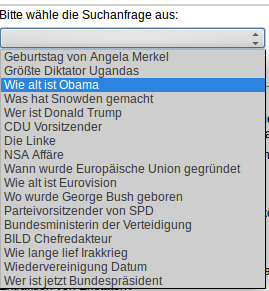
\includegraphics[width=.6\textwidth]{Bilder/select-question.png}
\caption{''Auswahl einer Frage''}
\label{fig:eval-select-question}
\end{figure}

Dabei wurden die Fragen in zwei Gruppen geteilt, um mögliche Abhängigkeit der Ergebnisse von dem Domain erkennen zu können - da verschiedene Engines und Modelle auf verschiedenen Korpora trainiert wurden, kann es sein, dass z. B. die Modelle, die auf Zeitungen trainiert wurden (TIGER Korpus), auch bei den Zeitung-ähnlichen Texten besser abschneiden werden. Es wurden folgende Gruppen von Fragen verwendet:
\begin{enumerate}
\item Die Fragen, die zum Domain ,,Zeitungen`` passen, was bedeutet, dass die Suchmaschinen bei der Beantwortung dieser Fragen höchstwahrscheinlich die Links auf Online-Zeitungen zurückgeben werden.
\item Die Fragen, die zum Domain ,,Web/Wikipedia`` passen, was bedeutet, dass die Suchmaschinen bei der Beantwortung dieser Fragen die Links auf Wikipedia zurückgeben sollen.
\end{enumerate} 
Um gleiche Bedeckung von allen möglichen Kombinationen von Domains und Fragegruppen zu gewährleisten, wird es bei jedem Engine zwischen verfügbaren Fragegruppen zyklisch gewechselt - für den ersten Benutzer wird die Reihenfolge 'Domain1/Engine1 $\longrightarrow$ Domain2/Engine2 $\longrightarrow$ Domain1/Engine3 ...' verwendet, für den zweiten 'Domain2/Engine1 $\longrightarrow$ Domain1/Engine2 $\longrightarrow$ Domain2/Engine3 ...' usw.

Nachdem Benutzer die gewünschte Frage ausgewählt und gestellt hat, wird ihm im zweiten Bereich, deren Schnappschuss auf der Abbildung \ref{fig:eval-entitylist} zu sehen ist, eine Liste von gefundenen Snippets mit den verlinkten Entitäten zusammen angezeigt.

Die Links auf die Webseiten und Snippets kommen dabei direkt von Bing, und werden damit von der Implementierung eines Engines nicht beeinflusst. Die Liste von Entitäten wird dagegen von dem Stanbol erstellt. Die Snippets, wo keine Entitäten gefunden werden konnten, werden in der Liste nicht angezeigt.

Im dritten Bereich (siehe die Abbildung \ref{fig:eval-props}) werden die Eigenschaften der ausgewählten Entität angezeigt. In der linken Spalte wird der Name der Eigenschaft abgebildet und rechts das Wert. Es gibt dabei zwei verschiedene Typen von Werten:
\begin{itemize}
\item ,,Rohe`` Eigenschaften, wie Geburts- oder Todesdatum oder Kurzbeschreibung. Diese sind im Prinzip Zeichenketten und können dem Benutzer ohne weiteres angezeigt werden.
\item ,,Links`` - das sind die Eigenschaften, die eigentlich nur Links auf andere Entitäten sind, die ihre eigene Eigenschaften besitzen. Zum Beispiel ist Geburtsort einer Person ein Link auf entsprechendes DBpedia-Eintrag, dasselbe gilt auch für Sprache oder sogar Zeitzonen.
\end{itemize}

Im letzten Bereich soll das getestete Engine bewertet werden, wie es auf der Abbildung \ref{fig:bewertung} angezeigt wird.

Nachdem alle Kombinationen getestet wurden, wird dem Benutzer die Möglichkeit gegeben, eine beliebige Frage an ein Engine zu stellen und einen persönlichen Feedback abzugeben. Die Aufbau dieser letzten Seite ähnelt sich der von der Seite, wo ein Engine bewertet wird, mit dem Unterschied, dass anstatt der Form für die Bewertung wird im letzten Bereich die Form für den Feedback und das Eingabefeld für die beliebige Frage angezeigt. Diese Änderung ist auf dem Screenshot \ref{fig:finish-eval} zu sehen. Diese Form wurde eingeführt, um die Anregungen für mögliche Verbesserungen vom Backend und für Nachfolgerarbeit sammeln zu können.

Während der Studie wurden insgesamt 44 Bewertungen gesammelt, deren Ergebnisse in der Tabelle \ref{app:RESULTS} zu sehen sind. Es wurden außerdem einige Feedbacks gesammelt, die für die Analyse der Arbeit und als Quelle für Verbesserungsvorschläge verwendet werden können. Die Liste von Feedbacks findet man in der Auflistung \ref{app:feedbacks}.

\begin{table}
\begin{tabular}{|c|c|c|c|c|}
\hline 
• & helpQuality & quality\_newspapers & quality\_misc & speed \\ 
\hline 
mitie-nerchain-pig & 3.23 & 1.98 & 1.45 & 4.09 \\ 
\hline 
mitie-nerchain-tiger & 3.15 & 1.25 & 2.09 & 3.8 \\ 
\hline 
pig-nerchain & 3.05 & 1.31 & 2 & 3.87 \\ 
\hline 
stanford-nerchain-both & 3.07 & 1.23 & 1.95 & 4.05 \\ 
\hline 
stanford-nerchain-dewac & 3.25 & 2.11 & 1.41 & 4.16 \\ 
\hline 
stanford-nerchain-hgc & 3.11 & 1.34 & 1.86 & 4.16 \\ 
\hline 
tiger-nerchain & 3.34 & 1.93 & 1.39 & 3.98 \\ 
\hline 
\end{tabular} 
\caption{Ergebnisse der Benutzerevaluierung}
\label{app:RESULTS}
\end{table}

Die Erklärung und Auswertung von den gesammelten Ergebnissen wird später in der Sektion ,,Diskussion`` (\ref{sec:diskussion}) vorgeführt. 

\section{Technische Implementierung der Benutzerevaluierung}
\paragraph{}
Die Komponentenstruktur der Evaluierungsseite ist auf der Abbildung \ref{fig:evalcomponents} dargestellt. Das System besteht insgesamt aus folgenden Komponenten:
\begin{enumerate}
\item Die Evaluierungswebseite selbst ist als eine Java-Webapplikation implementiert, und ist für die graphische Oberfläche verantwortlich.
\item Die Bing-API, die im Rahmen der Masterarbeit von Karatassis\cite{Karatassis:15} entwickelt wurde, stellt eine Schnittstelle zur Suche im Bing zur Verfügung.
\item MongoDB - eine dokumentenbasierte NoSQL-Datenbank - dient als Quelle für verfügbare Fragen und speichert außerdem die Bewertungen und Feedbacks von Benutzern.
\item Mit Hilfe der API für Extraktion von Entitäten greift die Webseite auf Stanbol, der auf einem anderen Rechner läuft, über eine REST-API zu. 
\end{enumerate}

\begin{figure}
\centering
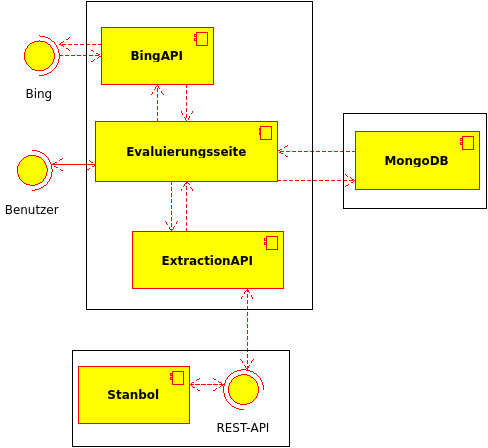
\includegraphics[width=1\textwidth]{Bilder/evaluation_components.png}
\caption{''Komponentendiagramm der Evaluierungsseite''}
\label{fig:evalcomponents}
\end{figure}
Der Vorteil dieser Architektur ist, dass die sich auf mehrere Rechnern verteilen lässt, womit die Verfügbarkeit und Belastbarkeit des System erhöht werden könnte.

Technische Details der Ablauf der Evaluierung werden auf der Diagramm \ref{fig:eval-ablauf} abgebildet. Der Vorgang der Evaluierung lässt sich in folgende Schritte aufteilen:
\begin{enumerate}
\item Zuerst wird die Anfrage des Benutzers an Web-Frontend gesendet.
\item Danach wird diese Anfrage an Bing weitergeleitet. Der BingAPI wird dabei mitgeteilt, dass bei Möglichkeit nur nach deutschsprachigen Webseiten gesucht werden muss.
\item Die Liste von Links auf gefundene Webseiten mit den Texten von Snippets zusammen, die vom Bing erhalten wurden, wird über ExtraktionAPI an Stanbol weitergeleitet.
\item Die von dem Stanbol erhaltene Antwort wird mithilfe von der ExtraktionAPI aus RDF in Java-Objekte transformiert.
\item Die Evaluierungsseite serialisiert extrahierte Entitäten, fügt die der vom Bing erhaltener Liste von Snippets zu und sendet die Ergebnisse an den Benutzer.
\item Der Benutzer benutzt Webseite-UI um das Engine zu bewerten.
\item Die Bewertung wird in der Datenbank gespeichert, und Benutzer kann mit dem nächsten Engine fortfahren.
\end{enumerate}

\begin{figure}
\centering
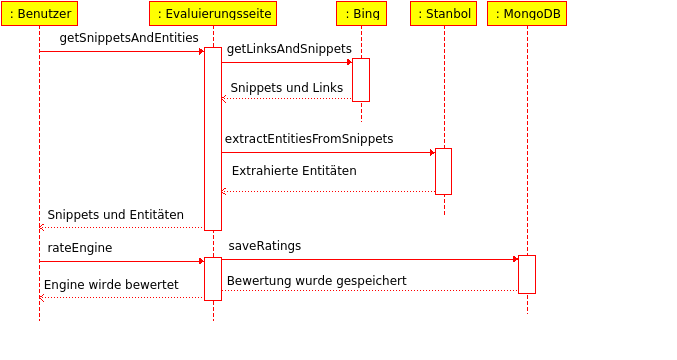
\includegraphics[width=1\textwidth]{Bilder/eval_sequence.png}
\caption{''Ablauf der Evaluierung''}
\label{fig:eval-ablauf}
\end{figure}

Die auf der Abbildung \ref{fig:evalcomponents} dargestellte Komponenten werden durch folgende Klassen implementiert:
\begin{itemize}
\item Das Interface \textit{EvaluationSessionService} und implementierende Klasse \textit{EvaluationSessionServiceImpl} sind für die Steuerung des Evaluierungsvorgangs zuständig:
\begin{itemize}
\item Die starten und beendet die Evaluierung für einen bestimmten Benutzer.
\item Die wechseln zum nächsten Engine, wenn der Benutzer die Bewertung abgeschickt hat.
\item Die leiten die Benutzerbewertungen und Anfragen zu anderen Komponenten weiter.
\end{itemize}
\item \textit{EingineRatingService} ist für die Speicherung von Benutzerbewertungen zuständig. Dabei definiert das Interface nicht, wie genau die Daten gespeichert werden - es muss also nicht unbedingt eine NoSQL datenbank sein - es wird nur eine generische Schnittstelle für Abgabe von Bewertungen zur Verfügung gestellt.
\item Die Klasse \textit{EingineRatingServiceMongoImpl} ist die Implementierung der \textit{EingineRatingService}-Schnittstelle für MongoDB.
\item \textit{MongoDbClient} stellt eine Abstraktion über die Mongo Java API zur Verfügung, damit es weniger Code für andere Klassen geschrieben werden müsste.
\item Die Klassen \textit{MongoFeedbackService} und \textit{AvailableQueriesFromDatabaseServiceMongoImpl} sind entsprechend für die Speicherung von Benutzerfeedbacks und möglichen Evaluierungsanfragen zuständig. 
\item \textit{EntityExtractionService} ruft zuerst Bing API (implementiert durch die Klasse \textit{BingSearchService}) auf, um die Liste von gefundenen Snippets für die angegebene Suchanfrage liefern zu lassen. Danach wird die Extraktion-API aufgerufen, um die gefundene Snippets mit Entitäten anzureichern. Die Ergebnisse werden zurück an \textit{EvaluationSessionService} geschickt.
\item Die Schnittstelle \textit{QueryLogService} und ihre Implementierung \textit{QueryLogServiceMongoImpl} sichern die Anfragen, die Benutzer im letzten Schritt der Evaluierung gesendet haben.
\end{itemize}

%\begin{figure}
%\centering
%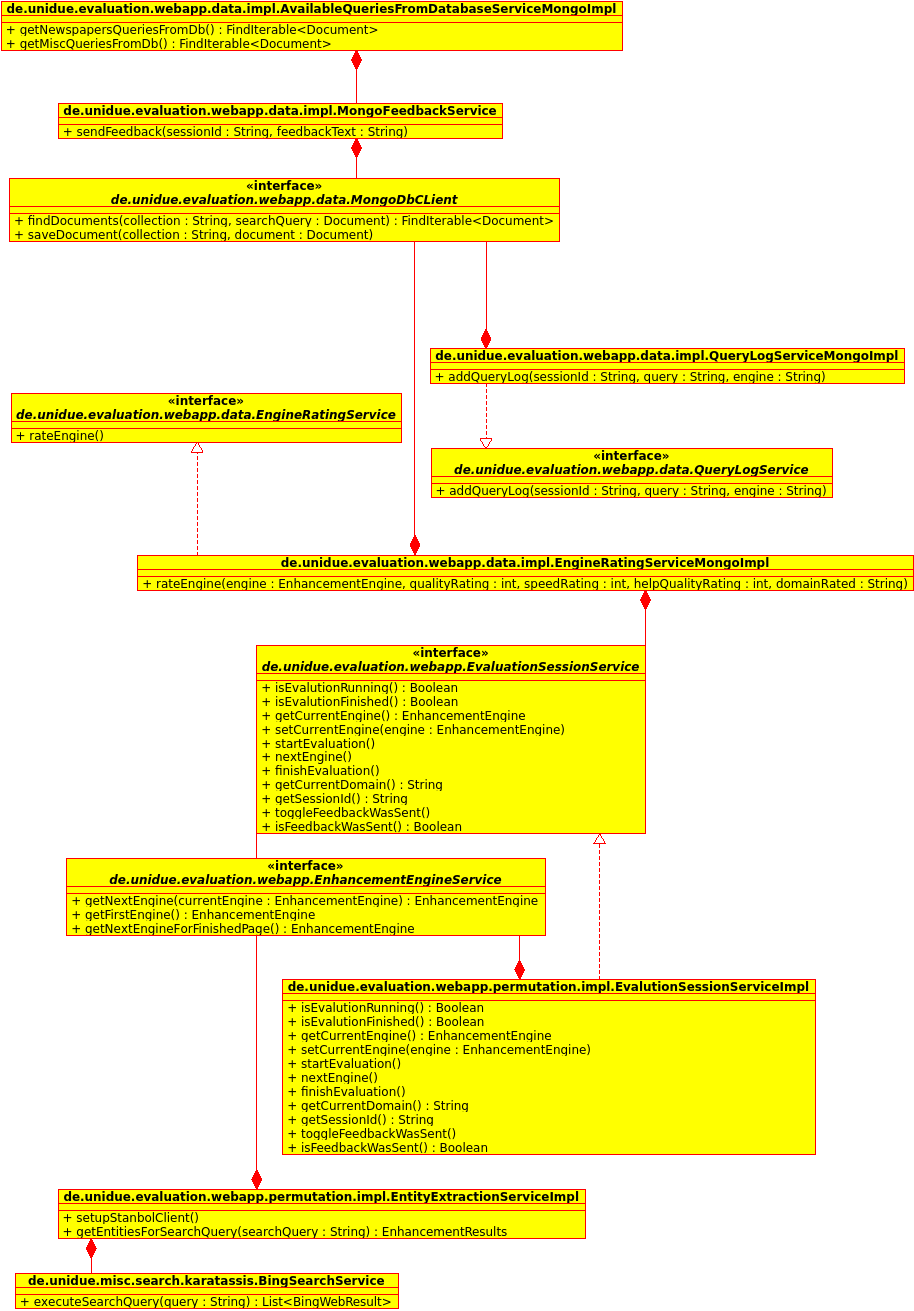
\includegraphics[width=1\textwidth]{Bilder/eval_classes.png}
%\caption{''Klassendiagramm der Evaluierungsseite''}
%\label{fig:evalclasses}
%\end{figure}

Genau wie Stanbol kann die Evaluierungsseite auf jedem Java Applikationsserver gestartet werden. Es ist möglich, dass die Seite eine Java VM mit Stanbol teilt, was allerdings aus Geschwindigkeitsgründen nicht empfohlen wird.

\section{Systemorientierte Evaluierung von Qualität der Extraktion} \label{sec:sysevalsec}
\paragraph{}
Bevor die Ergebnisse der Benutzervaluierung bewertet werden können, muss geprüft werden, wie präzis die Engines Entitäten erkennen können. Da ein Engine in seiner Funktionsweise ein Klassifikator ist (siehe Kapitel ,,Grundlagen``, Sektion \ref{sec:Grundlagen}), kann die Präzision eines Engines anhand von folgenden Metriken bestimmt werden\footnote{\url{https://de.wikipedia.org/wiki/Beurteilung_eines_Klassifikators\#Wahrheitsmatrix:_Richtige_und_falsche_Klassifikationen} (Zuletzt abgerufen am 05. November)}
\begin{enumerate}
% dund  (die Wörter, die keine Entitäten sind, und die nicht als Entitäten annotiert wurde) definiert werden.
\item Anzahl von False-Positive-Treffer - die von dem Engine als Entitäten erkannte Wörter, die keine Entitäten sind.
\item Anzahl von True-Positive-Treffer - die Entitäten, die von dem Engine als solche erkannt wurden.
\item Anzahl von True-Negative-Treffer - die Wörter, die keine Entitäten sind, und die als solche nicht annotiert wurden.
\item Anzahl von False-Negative-Treffer - die von dem Engine nicht erkannte Entitäten.
\end{enumerate}

Die oben genannte Zahlen können mithilfe von folgenden Metriken zusammengefasst werden\cite{och2003systematic}:
\begin{itemize}
\item Präzision beschreibt den Anteil von True-Positive-Treffer an allen als Entitäte markierten Wörtern (die Summe von True-Positive- und False-Positve-Treffer).
\item Sensitivität (Recall) beschreibt den Anteil von korrekt als Entitäte erkannten Wörtern (True-Positive-Treffer) an den Anzahl von allen im Text vorhandenen Entitäten (Die Summe von True-Positive-Treffer und False-Negative-Treffer).
\item F-Measure fasst Präzision und Sensitivität mithilfe des gewichtetes harmonisches Mittels zusammen. Die Formel für die Kalkulation von F-Maß für Präzision $P$ und Sensitivität $S$ sieht wie folgt aus\cite{hripcsak2005agreement}:
$$
F=\frac{(1+\beta^2)*S*P}{(\beta^2*P)+S}
$$ 
Die Variable $\beta$ bestimmt dabei, was ein höheres Gewicht für die Kalkulation des F-Wertes hat: Präzision oder Sensitivität. Allerdings sollen diese beide Maßen in meisten Fällen laut Hripcsak\cite{hripcsak2005agreement} gleiches Gewicht besitzen, und so kann das Gewicht $\beta$ auf $1$ gesetzt werden.
\end{itemize}

Nachdem die Maßen, die für jedes Engine berechnet werden sollen, definiert wurden, muss ein Verfahren zur Beurteilung von Engines bestimmt werden (das bedeutet, dass es eine Methodik ausgewählt werden soll, die bestimmt, wie die Evaluierung durchgeführt werden soll). In der Arbeit von Kovahi et al.\cite{kohavi1995study} wurde erwähnt, dass zur Bewertung von Klassifikatoren Kreuzvalidierung verwendet werden soll. Allerdings kann die Kreuzvalidierung nicht auf alle Engines angewendet werden, da es für einige Engines keine Trainingskorpora zur Verfügung stehen, wie es im Kapitel ,,Implementierung`` (Sektion \ref{subsec:stanfordner}) erwähnt wurde. Aus diesem Grund wird in dieser Masterarbeit folgende Evaluierungsmethodik verwendet:
\begin{itemize}
\item Als Musterdaten für die Evaluierung wurden TIGER- und PIG-Korpora verwendet:
\begin{itemize}
\item Die Engines, die mithilfe von PIG trainiert wurden, werden mit dem TIGER-Korpus ausgetestet.
\item Die Engines, die mithilfe von TIGER trainiert wurden, werden mit dem PIG-Korpus ausgetestet.
\item Auf Stanford-NER aufgebaute Engines wurden mithilfe von PIG-Korpus getestet, da er größer ist, und da die Varianz von Daten dort größer sein soll, und so theoretisch genauere Ergebnisse liefern könnte.
\end{itemize}
\item Die Anfragen werden direkt an eine Stanbol-Instanz mithilfe der REST-API gesendet.
\end{itemize}
Auf diese Art und Weise wird nicht nur die Qualität von den verwendeten Modellen bewertet, sondern auch andere Bestandteile von Engines, wie Filter von Entitäten und Verlinkung- und Dereferenzierungsengines.

Die Ergebnisse dieser systemorientierter Evaluierung sind in der Tabelle \ref{tab:AUTOEVAL} aufgelistet. Es lässt sich gut erkennen, dass die Ergebnisse sich mit den im Kapitel ,,Grundlagen`` (Sektion \ref{sec:Grundlagen}) gemachten Annahmen gut vereinbaren lassen - das Engine, das SVM als Basisalgorithmus verwendet (MITIE), zeigt auch die beste Ergebnisse. Aber wie gut spiegeln diese Daten die ,,Zufriedenheit`` der Benutzer mit dem Engine? Auf diese Frage wird während der Diskussion von Ergebnissen (\ref{sec:diskussion}) angegangen.

\begin{table}
\begin{tabular}{|c|c|c|c|}
\hline 
• & F-Measure & Recall & Präzision \\ 
\hline 
MITIE (PIG) & 0.585 & 0.506 & 0.693 \\
\hline
OpenNLP (PIG) & 0.404 & 0.299 & 0.621 \\
\hline
STANFORD (deWac+hgc) & 0.246 & 0.187 & 0.359 \\
\hline
STANFORD (deWac) & 0.280 & 0.219 & 0.390 \\
\hline
STANFORD (hgc) & 0.271 & 0.209 & 0.388 \\
\hline 
MITIE (TIGER) & 0.557 & 0.624 & 0.503 \\
\hline
OpenNLP (TIGER) & 0.409 & 0.357 & 0.479 \\
\hline
\end{tabular} 
\caption{Ergebnisse der systemorientierten Evaluierung}
\label{tab:AUTOEVAL}
\end{table}

\section{Diskussion} \label{sec:diskussion}
\paragraph{}
Nachdem sowohl system- als auch benutzerorientierte Evaluierungen durchgeführt wurden, können die Ergebnisse zusammengefasst und erklärt werden. Auf den ersten Blick lassen sich aus den vorgestellten Ergebnissen folgende Schlussfolgerungen ziehen:
\begin{itemize}
\item Die Benutzer fanden den Einsatz hilfreich, wünschen sich aber die Verbesserung von dem Benutzerinterface des Systems.
\item Es werden eventuell zu viel Informationen angezeigt, so dass der Benutzer sich verwirrt fühlen könnte.
\item Die Probanden fanden die Geschwindigkeit der Suche gut, auch wenn es definitiv länger als eine Suche mit herkömmlichen Suchmaschinen dauert. 
\item Die Benutzer bewerteten die Qualität von extrahierten Entitäten meistens als ,,nicht ausreichend``.
\item Obwohl die automatisierte Evaluierung von Engines klare Ergebnisse geliefert hat, und zwar, dass ein Engine viel bessere Ergebnisse gezeigt hat, als die andere, wird das in der Benutzerevaluierung nicht widergespiegelt.
\end{itemize}

Es stellt sich die Frage, was bedeuten diese Ergebnisse, und was man daraus lernen kann, und welche Aspekte des entwickelten Systems sich verbessern lassen.

Die interessanteste Frage wäre, warum die Benutzer einerseits die Qualität von den extrahierten Entitäten als ,,schlecht`` bewertet haben, aber anderseits den Einsatz von Entitäten als ,,hilfreich`` bezeichneten, und welchen Zusammenhang zwischen diesen beiden Kriterien besteht? 

Um diese Frage beantworten zu können muss es zuerst über die Definition von ,,Qualität`` von Entitäten im Rahmen der Evaluierung nachgedacht werden. In der Einleitung zur Evaluierung wurde Qualität als ,,wie gut \textbf{aus Sicht des Probanden} die Entität zu den gefundenen Snippets passt`` definiert. Das Problem hier ist, dass verschiedene Benutzer verschiedene persönliche Definitionen von den Begriffen ,,passend`` und ,,unpassend`` haben - z.B. wird aus einem Snippet zur Anfrage ,,Geburtstag von Angela Merkel`` auch die Entitäten ,,Deutschland`` und ,,CDU`` extrahiert, neben der Entität ,,Angela Merkel``, die für die Beantwortung der Anfrage eigentlich ausreichend wäre. Einige Probanden können die zwei zusätzliche Entitäten als ,,passend`` einstufen, da die zum Themengebiet des Snippet-Textes passen, aber andere Benutzer würden dieselbe Daten als ,,unpassend`` bezeichnen, da die keine Antwort auf die gestellte Frage geben. Außerdem sind die Methoden zur Extraktion von Entitäten nicht perfekt, und können im Text vorhandene Entitäten nicht immer richtig erkennen. Die Rolle vom Trainingskorpus soll auch im Kauf genommen werden - automatisch generierte Korpora sollen generell nur dann verwendet werden, wenn keine weitere Korpora verfügbar sind (aus finanziellen Gründen z.B.).

Ein weiteres Problem kann auf die Suchmaschine zurückgeführt werden, die als Quelle für Snippets verwendet wird - auch wenn in den Suchparametern der Suchmaschine explizit mitgeteilt wird, dass es nach deutschsprachigen Seiten gesucht werden muss, werden oft auch englischsprachige Webseiten gefunden, und da das im Rahmen dieser Arbeit entwickeltes System nur für deutsche Sprache funktionieren soll, werden nicht alle von der Suchmaschine erhaltene Ergebnisse mit den Entitäten angereichert.

Die Andere Quelle für die Bewertung von extrahierten Entitäten als ,,unpassend`` können die in den dem Benutzer gezeigten Ontologien vorhandene Informationen sein. Als Erstes haben einige Benutzer bemerkt, dass es auch die Eigenschaften angezeigt werden, die mit der eigentlichen Suchanfrage nichts gemeinsames haben - z.B. auch wenn man die Informationen übers Geburtsort einer Person sucht, werden für die extrahierte Entität alle in der Wissendatenbank vorhandene Informationen angezeigt - Geburtstag, Name, Beschreibung u.s.w. Das kann zur Verwirrung führen, und somit wird die Entität als ,,schlecht`` eingestuft. Zweitens, sind die in DBpedia vorhandene Daten nicht immer vollständig - bei den Daten fürs indische Ozean fehlen z.B. die Angaben zur Fläche, da die direkt in der Kurzbeschreibung der Entität zu finden sind. Das kann eventuell dazu führen, dass der Benutzer sich in die Beschreibung der extrahierten Entität einlesen muss, und somit mehr Aufwand für die Suche anzuwenden braucht als es vorgesehen wurde. 

Ein weiterer Grund, warum die Entitäten als ,,nicht ausreichend gut`` bewertet wurden, könnte das User-Interface des Bewertungssystems sein - da das Ziel dieser Arbeit die Entwicklung des Backeds und der API für die Extraktion von Entitäten aus Suchergebnisseiten war, und die UI nur für die Durchführung der Evaluierung entwickelt wurde, wurde eine grundlegende Untersuchung, wie die Daten dem Benutzer am Besten angezeigt und dargestellt werden könnten, absichtlich nicht durchgeführt, damit der Zeitplan eingehalten werden könnte. Und obwohl es gebeten wurde, nicht die UI, sondern nur die Extraktion von Entitäten an sich selbst zu bewerten, beeinflusst die UI die Entscheidung des Benutzers trotzdem. 

Die mögliche Schreibfehler sowohl in den Anfragen von Benutzern als auch in den Texten von gefundenen Snippets müssen auch im Kauf genommen werden - das System hat zur Zeit keine Möglichkeit, Schreibfehler zu korrigieren, was dazu führen kann, dass einige vorhandene Entitäten nicht gefunden werden.

Anschließend könnte auch die Komplexität der Evaluierungsseite an sich selbst auf den Benutzer verwirrend wirken, und so für schlechtere Wahrnehmung der Ergebnissen sorgen.

Der Grund für die Unstimmigkeiten zwischen der Benutzer- und automatisierten Evaluierung könnte die Tatsache sein, dass für den Benutzer \textbf{die in den Entitäten vorhandene Daten}, wie Geburtsort, viel wichtiger, als die Entitäten selbst sind - auch wenn eine Entität aus dem Text extrahiert wurde, kann die für den Benutzer ohne verlinkte Eigenschaften nicht nützlich sein.
